
Rust Part

Rust的所有权模型是其编译时内存安全和管理的关键。所有权基于仿射类型,其中一个值最多只能使用一次。在Rust中,每个值都有一个所有者,例如,下面的代码中分配的字符串值“hello!”由hello变量拥有。在一个值被移动之后,例如,如果“hello!”在第5行中被从hello移动到owned\_string (第14行),它的所有权将被转移,之前的所有者(hello)将不能再使用它。

\begin{lstlisting}[caption=Rust Demo, numbers=left]
fn main() {
	let hel: &str;
	{
		let hello = String::from("hello!");
		// consume(hello); // -> "value moved" error in here.
		let borrowed_str: &str = &hello;
		hel = substr(borrowed_str);
		// println!("{}", hel); // -> lifetime error
	}
}
fn substr<'a> (input_str: &'a str) -> &'a str {
	&input_str[0..3] // return value has lifetime 'a
}
fn consume(owned_string: String) { }
\end{lstlisting}


当所有者的作用域结束时,例如,在词法块的末尾,通过编译器插入对其析构函数的调用,所有者的值将被丢弃(释放)。Rust中的析构函数是通过实现给定类型的Drop特征来实现的,其中自定义的Drop处理程序可以执行除释放内存之外的任意操作。在上面的第8行中,hello字符串超出了作用域,并由它的删除处理程序自动释放。

还可以通过 borrow 来获得对它们的引用(第6行),而且这些引用的生命周期不能超过所拥有值的生命周期。第11行中的语法将input\_str参数的生命期命名为'a,并指定返回的\&str引用具有相同的生命期'a。返回的\&str引用在第7行中被赋值给hel,这将在第9行中由于生命周期的原因而被释放,因为在第8行中,hel将在它最初从(hello)借来的拥有值被删除后使用。Rust的编译器包括一个借用检查器来执行这些生命周期规则,以及别名异或可变性的核心原则,其中可以有多个不可变引用,也可以有单个对值的可变引用,但不能同时存在这两个引用。这允许它静态地确保堆栈和堆上的值的内存安全。

系统设计还广泛利用了Rust泛型的特征,是一种抽象类型的声明,它指定了类型必须实现的方法集,类似于OOP语言中的多态接口。trait可用于在泛型类型参数上设置边界。例如,函数fn print\_str<T: Into<String>>(s: T){},其中<T: Into<String>约束了入参s的类型,其必须实现Into<String>的泛型特征, 如果s没有符合类型约束则在代码编译时就会被抛出错误。


Riscv Part

RISC-V\pagescite{riscv0}指令集是基于精简指令集计算(RISC)原理建立的开放指令集架构(ISA),RISC-V是在指令集不断发展和成熟的基础上建立的全新指令。RISC-V指令集是开源的,由于设计简单,该指令集易于移植。Riscv的模块化设计和完整的开发工具链,使其拥有大量的开源实现和流片。由于操作系统依赖于底层的指令集设计规范,因此需要提前知晓Riscv的机器模式和其比较典型的内存设计方案Sv39\pagescite{xv60}的地址个俗称
\subsubsection{Riscv的机器模式}

指令集定义了3种特权模式(机器模式(M), 监督模式(S), 用户模式(U)),从而实现了空间和指令安全。\pagescite{riscv0}

指令架构约定机器模式为必选,另外两种模式则可选,通过模式的模块组合可以实现不同的指令组织形式。\pagescite{riscv0}其中M拥有最高的权限,而U的权限则是最低的,权限高的模式对于权限低的模式是透明的,权限低的无法获得权限高的所拥有的资源。从而达到了层与层之间的隔离,设计上指令集是安全的。

SBI(Supervisor Binary Interface)是Supervisor Execution Environment (SEE)和supervisor之间的接口。 它允许监督者层通过调用 ecall 指令执行一些特权操作。 SEE 和 supervisor 的示例有:类Unix平台上的机器模式和监督者模式,其中 SBI 是它们之间的一层接口,且是唯一,以及 Hypervisor extended-Supervisor (HS) 和 Virtualized Supervisor (VS)。

\subsubsection{Sv39}

\textbf{地址格式与组成}

\begin{figure}[htb]
    \figureCapSet
    \centering
    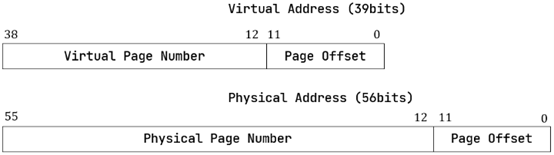
\includegraphics[width=.8\linewidth]{figure/c2/addressstructure.png}
    \caption{Sv39的地址格式}
    \label{figure:c2addressstructure}
\end{figure}

采用分页管理,单个页面的大小设置为 4KiB ,每个虚拟页面和物理页帧都对齐到这个页面大小,也就是说虚拟/物理地址区间 [0,4KiB) 为第 0 个虚拟页面/物理页帧,而 [4KiB,8KiB) 为第 1 个,以此类推。 4KiB 需要用 12 位字节地址来表示,因此虚拟地址和物理地址都被分成两部分:它们的低 12 位,即 [11:0] 被称为 页内偏移 (Page Offset) ,它描述一个地址指向的字节在它所在页面中的相对位置。\pagescite{xv60}而虚拟地址的高 27 位,即 [38:12] 为它的虚拟页号 VPN,同理物理地址的高 44 位,即 [55:12] 为它的物理页号 PPN,页号可以用来定位一个虚拟/物理地址属于哪一个虚拟页面/物理页帧。

地址转换是以页为单位进行的,在地址转换的前后地址的页内偏移部分不变。\pagescite{xv60}可以认为 MMU 只是从虚拟地址中取出 27 位虚拟页号,在页表中查到其对应的物理页号(如果存在的话),最后将得到的44位的物理页号与虚拟地址的12位页内偏移依序拼接到一起就变成了56位的物理地址。\pagescite{riscv0}


\textbf{地址转换过程}

\begin{figure}[htb]
    \figureCapSet
    \centering
    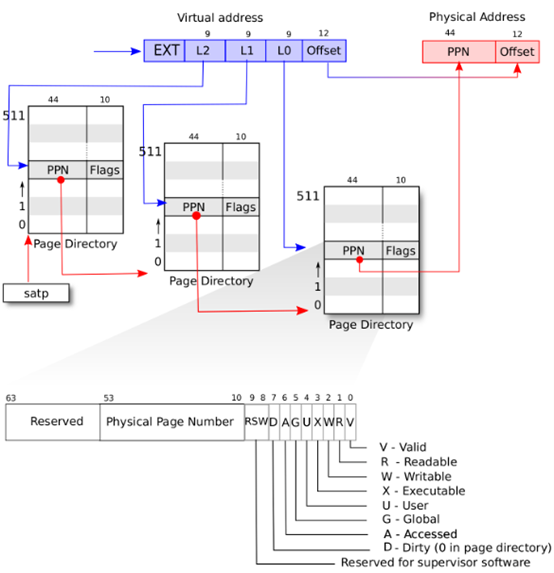
\includegraphics[width=.8\linewidth]{figure/c2/addressv2p.png}
    \caption{Sv39地址转换过程}
    \label{figure:c2addressv2p}
\end{figure}

在 SV39 模式中,采用三级页表,即将 27 位的虚拟页号分为三个等长的部分,第 26-18 位为一级页索引 virtualPageNumber0 ,第 17-9 位为二级页索引 virtualPageNumber1 ,第 8-0 位为三级页索引 virtualPageNumber2 。\pagescite{riscv0}

页表分为一级页表(多级页表的根节点),二级页表,三级页表(多级页表的叶节点)。每个页表都用 9 位索引,因此有 $2^9=512$ 个页表项,而每个页表项都是 8 字节,因此每个页表大小都为 $512\times 8=4 \mathrm{KiB}$,正好是一个物理页的大小。\pagescite{riscv0}从而可以把一个页表放到一个物理页中,并用一个物理页号来描述它。事实上,一级页表的每个页表项中的物理页号可描述一个二级页表;二级页表的每个页表项中的物理页号可描述一个三级页表;三级页表中的页表项内容则和先前提到的页表项一样,包含物理页号,即描述一个要映射到的物理页。\pagescite{riscv0}

% TODO: could not fix.
具体来说,假设虚拟地址的格式为:
\begin{equation}
    \label{equation:c2vpn}
    \begin{aligned}
        (virtualPageNumber_{0} ,virtualPageNumber_{1},virtualPageNumber_{2},offset)
    \end{aligned}
\end{equation}
	系统的内存,首先会装载,当前所用的一级页表的物理页的页号到 satp 寄存器中;
    \begin{itemize}
	\item 把 $virtualPageNumber_{0}$ 作为偏移量在一级页表的物理页中找到二级页表的物理页号;\pagescite{xv60}
	\item 把 $virtualPageNumber_{1}$ 作为偏移量在二级页表的物理页中找到三级页表的物理页号;\pagescite{xv60}
	\item 把 $virtualPageNumber_{2}$ 作为偏移量在三级页表的物理页中找到要访问位置的物理页号;\pagescite{xv60}
    \end{itemize}

物理页号对应的物理页基址(即物理页号左移12位)加上偏移量就是虚拟地址对应的物理地址。

处理器通过如此反复转换,从虚拟页号找到了一级页表项,得出了物理页号和虚拟地址所对应的物理地址。\pagescite{rcore0}若页表项满读写执行的标记都为 0,表明这个页表项指向下一级页表。\pagescite{rcore0}在这里三级和二级页表项的读写执行 为0应该成立,因为其指向了下一级页表。


\subsection{API与ABI}

从使用操作系统的角度会比较容易对操作系统内核的功能产生初步的认识。系统内核提供各种服务,其客体是运行在其所形成的执行环境中的应用程序,而系统使用者是通过应用程序的服务间接获得内核的服务,因此系统内核在一般用户面前是透明的。而应用程序需要访问内核获得其的服务,而这需要通过操作系统的调用接口才能完成,即应用程序二进制接口 (ABI, Application Binary Interface)。

操作系统往往不会供单一函数库的编程接口 (API, Application Programming Interface) ,它的接口需要考虑应用需求,访问安全等因素,使得应用软件不能像访问函数库一样的直接访问操作系统内部函数,更不能直接读写操作系统内部的地址空间。为此,操作系统设计了一套安全可靠的二进制接口,即系统调用接口, 其通常面向应用需求提供了API的描述,而具体实现,则需要遵循ABI的接口规范。\pagescite{rcore0}

在处理器和指令集合的支持(特权级隔离,内存空间隔离等)下,应用无需直接以函数调用的方式操作系统,读写底层。\pagescite{rcore0}不同类型的应用服务可以通过ABI和API的组合,提出服务请求,获得系统的服务。操作系统提供完服务后,返回应用程序继续执行。

API与ABI在设计层面上有非常多的相似之处,但是,为了明确系统编程的需求,还是将两者的区别提一下。

\subsubsection*{编程接口与二进制接口的区别}

二进制接口是不同特权级的连接纽带。ABI定义了二进制机代码的规则,包含了数据类型、通用寄存器、参数传递、以及堆栈等。二进制接口的设计基于处理器和内存地址等硬件架构,用来约束链接器和汇编器 。\pagescite{rcore0}同一处理器,基于不同高级语言编写的应用程序、库和操作系统,如遵循同样的ABI定义,那么就能被正确链接和执行。\pagescite{rcore0}

应用程序编程接口是源代码级别的连接纽带。API定义了一个源码级函数,类型,返回值等。因此API是用来约束编译器的:一个API是给编译器的指令,规定源代码的服务范围。\pagescite{rcore0}API与编程语言相关,如libc是基于C编写的标准库,那么C的应用程序就可以通过编译器与libc建立联系,并能正确访问libc中的函数。


在异步调用的时候,喝牛奶时,可以返回Futre,牛奶的工作会被置换到后台,然后掉起啃面包的行为,这个动作同样是异步的,换句话说,当面包的工作出现阻塞时,面包同样可以被置换到后台,让出资源。这样的工作使得相应函数可以更早地被执行,然后形成宏观上相应动作地并发执行,而无需在接收函数返回之前长时间的等待。

\subsection{Rust中的Future}

\begin{figure}[htbp]
    \figureCapSet
	\centering
	\begin{minipage}{0.49\linewidth}%表示图片的占用那一列的宽度
		\centering
\begin{lstlisting}[frame=none]
pub trait Future {
    type Output;
    fn poll(self: Pin<&mut Self>, cx: &mut Context) -> Poll<Self::Output>;
}
\end{lstlisting}
	\end{minipage}
    \hfill
	%\hfill表示横向排,两张图片会自动保证一定的距离
    %\vfill表示自动排版,两张图片会自动保证一定的距离
    %或者直接在这里加空格来增加图片之间的距离
	\begin{minipage}{0.49\linewidth}
		\centering
        \begin{lstlisting}[frame=none]
pub enum Pool<T> {
    Ready(T),
    Pending,
}
        \end{lstlisting}
	\end{minipage}
    \caption{Rust's Future}
\end{figure}

在上述的代码中,Future的trait接口,Output将会被返回一个异步的值。例如在时序图中提到的async\_eat\_milk的返回值。 而poll函数返回的是一个可以被轮询检查自身状态的值,其具体的结构如上图右部分。 

当poll返回的值Ready(T)时,函数将完成的值进行Poll的封装,返回其状态完成的变体。否则,将返回其其他状态的变体,向其范围内全局的调用者发出该工作尚未完成的信号。

poll方法接收两个参数: Pin(固定地址空间)和Context(函数上下文)。前者的行为类似普通引用,只是将值固定到内存的位置。后者存在的目的时为了Waker的实例可以被异步任务接收。这使得异步任务可以发出信号,表面其此时的状态(完成或一部分已完成)。由于主任务知道其将在准备就绪时收到通知,因此不需要一遍一遍调用。

\subsection{Future使用的例子}

下面的代码可以看成是早餐的Rust伪码描述,伪码中省略了不必要的细节,只给了能够说明问题的框架

\begin{lstlisting}[ caption = BREAKFIRST ]
enum FoodState {
    Cooked,
    Eating,
    Finished,
};
async fn milk () { /* ... */ }
async fn bread () { /* ... */ }
async fn eat () {
    /* ... */
    milk.await;
    bread.await;
    /* ... */
}

\end{lstlisting}

根据异步的设计规范,上述的代码,编译器将依赖状态转换,如\autoref{figure:c2breakfirststate},实现相应的状态保存和状态转换。

\subsubsection{状态转换}

在编译器的后台,上述的代码将会被转化为状态机,每个调用将会形成不同的状态,根据上述代码可以转化出下面的状态。每个状态表示函数中不同的暂停点。“开始”和“结束”状态表示函数在其执行的开始和结束时。“Waiting on Milk”状态表示函数当前正在等待第一个结果。同样,“Waiting on Bread”状态表示函数等待第二个结果的暂停点。状态机通过使每个调用成为可能的状态转换变为Rust的Future。

\begin{figure}[htb]
    \figureCapSet
    \centering
    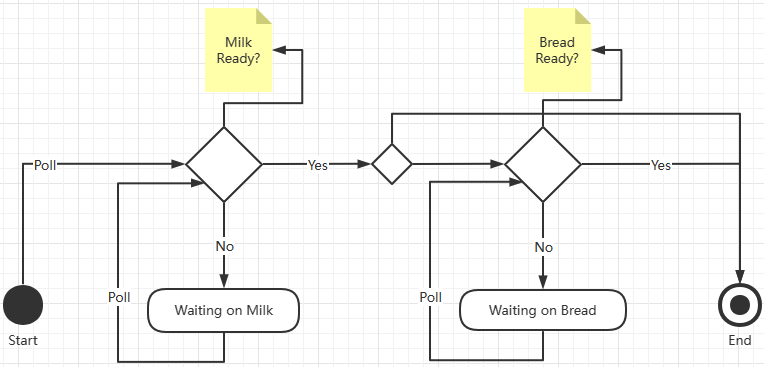
\includegraphics[width=.8\linewidth]{figure/c2/breakfirststate.png}
    \caption{Breakfirst的状态机图}
    \label{figure:c2breakfirststate}
\end{figure}

该图使用箭头表示状态开关,使用菱形表示替代方法。该图使用箭头表示状态开关,使用菱形表示替代方法。例如,牛奶没有喝完,则采用标记为“no”的路径,并达到“Waiting on Milk”状态。否则,将采用“是”路径。没有标题的小红色菱形表示函数eat的分支。

我们看到第一次调用启动函数poll并让它运行,直到它到达尚相应的状态。如果路径上的所有状态都准备就绪,则该函数进入“结束”状态,此状态中,函数返回会被 Poll::Ready包裹。否则,状态机将进入由Poll::Pending包裹的状态中。在下一次调用时,状态机将从等待状态开始,并反复上次操作。


\subsubsection{状态保存}

为了能够从上一个等待状态继续,状态机必须在内部跟踪当前状态。此外,它必须保存下次调用时继续执行所需的所有变量。这就是编译器真正可以发光的地方:因为它知道何时使用哪些变量,因此它可以自动生成具有所需变量的结构。

\begin{figure}[htbp]
    \figureCapSet
	\centering
	\begin{minipage}{0.49\linewidth}%表示图片的占用那一列的宽度
		\centering
        \begin{lstlisting}[frame=none]
async fn eating(min_energy: usize) -> String {
    let food = async_eat_milk().await;
    if food.energy() < min_energy {
        content + &async_eat_bread().await
    } else {
        content
    }
}
        \end{lstlisting}
	\end{minipage}
    \hfill
	%\hfill表示横向排,两张图片会自动保证一定的距离
    %\vfill表示自动排版,两张图片会自动保证一定的距离
    %或者直接在这里加空格来增加图片之间的距离
	\begin{minipage}{0.49\linewidth}
		\centering
        \begin{lstlisting}[frame=none]
enum BreakfirstStateMachine {
    State(StartState),
    WaitingOnMilk(WaitingOnMilkState),
    WaitingOnBread(WaitingOnBreadState),
    End(EndState),
}
        \end{lstlisting}
	\end{minipage}
    \caption{Breakfirst的状态机描述和与之对应的可能状态}
\end{figure}


在编译器中, 可以尝试这样理解, eating函数将会生成上图右边的状态。在Start和WaitingOnMilk的状态下,需要将参数存储下来,为food.energy()和min\_energy的对对比做准备。WaitingOnMilk的状态将会被WaitingOnMilkState所记录,其将会被全局的调度器所调用。当状态机继续运行时,async\_eat\_milk需要再次轮询WaitingOnMilkState,因此需要保存它。

为了使得描述方便, 每个状态都被定义一个单独的枚举变体(如上图右半部分),并将相应的状态结构作为字段添加到每个变体中。为了实现状态转换,编译器基于以下函数生成特征的实现:

\begin{lstlisting}[caption=Breakfirst的状态转换]
impl Future for BreakfirstStateMachine {
    type Output = String;
    fn poll(self: Pin<&mut Self>, en: &mut Energy) -> Poll<Self::Output> {
        loop {
            match self {
                BreakfirstStateMachine::Start(state) => {}
                BreakfirstStateMachine::WaitingOnMilk(state) => {}
                BreakfirstStateMachine::WaitingOnBread(state) => {}
                BreakfirstStateMachine::End(state) => {}
            }
        }
    }
}
\end{lstlisting}

Future的类型是因为它是函数的返回类型。为简单起见,我们只显示简化的代码,不处理Pin、所有权、生存期等。因此,此代码和以下代码应被视为伪代码,而不是直接使用。当然,真正的编译器生成的代码可以正确处理所有内容,尽管可能以不同的方式处理。


为了使代码摘录保持较小,我们分别显示每个臂的代码。让我们从Start状态开始

\begin{lstlisting}[caption = Start Branch]
BreakfirstStateMachine::Start(state) => {
    let eat_milk_future = async_eat_milk();
    let state = WaitingOnMilkState {
        min_energy: state.min_energy,
        eat_milk_future,
    }
    *self = BreakfirstStateMachine::WaitingOnMilk(state);
}
\end{lstlisting}

状态机处于函数开头的状态Start。在这种情况下,执行从函数体到第一个.await为了处理该操作,将状态机的状态更改为WaitingOnMilk,其中包括结构的构造。


由于语句是在循环中执行的,因此执行跳转到接下来的状态:

\begin{lstlisting}[caption=WaitingOnMilk Branch]
BreakfirstStateMachine::WaitingOnMilk(state) => {
    match state.eat_milk_future.poll(en) {
        Poll::Pending => return Poll::Pending,
        Poll::Ready(energy) => {
            if food.energy() < state.min_energy {
                let eat_bread_future = async_eat_bread();
                let state = WaitingOnBreadState {
                    energy,
                    eat_bread_future,
                }
                *self = BreakfirstStateMachine::WaitingOnBread(state);
            } else {
                *self = BreakfirstStateMachine::End(EndState);
                return Poll::Ready(energy);
            }
        }
    }
}
\end{lstlisting}

在这个分支中,首先调用Poll::Pending如果还没有准备好,我们退出循环并返回self, 由于在这种情况下保持该状态 WaitingOnMilk,因此状态机上的下一个调用将进入同一分支并再次轮询。

准备就绪后,我们将结果分配给变量并继续执行函数的代码: 如果小于保存在状态结构中的值,则异步开始啃食面包。此时再次将操作转换为状态更改,这次转换为WaitingOnBread状态。由于正在执行内部循环,因此执行之后直接跳转到新状态的分支,然后再次轮询。

如果我们进入条件的另一条分支,则不会发生进一步的操作。从而到达函数的末尾并返回包装在 Poll::Ready,并将当前状态更改为End状态。


WaitingOnBread的代码如下:

\begin{lstlisting}[caption=WaitingOnBread Branch]
BreakfirstStateMachine::WaitingOnBread(state) => {
    match state.async_eat_bread.poll(en) {
        Poll::Pending => return Poll::Pending,
        Poll::Ready(bread_energy) => {
            *self = BreakfirstStateMachine::End(EndState);
            return Poll::Ready(state.energy + &bread_energy);
        }
    }
} 
\end{lstlisting}
与状态WaitingOnMilk类似,我们首先轮询async\_eat\_bread如果它仍然挂起,我们退出循环并返回Poll::Pending否则,我们可以执行函数的最后一个操作:将变量与将来的结果连接起来。我们将状态机更新为End状态,然后返回包装在Poll::Ready中的结果。

最后的代码为

\begin{lstlisting}[caption=End Branch]
BreakfirstStateMachine::End(state) => {
    panic!("poll called after Poll::Ready was returned");
} 
\end{lstlisting}
Future返回后不应再次轮询,因此,如果在对于已经处于该状态时被调用,编译器应当抛出panic。